\selectlanguage{greek}
\chapter{Ανάπτυξη του \en{GraKeL}}
\label{chap3}
Η σχεδίαση μίας μοντέρνας βιβλιοθήκης προγραμματισμού δεν είναι μία απλή υπόθεση.
Ο προγραμματιστής καλείται να συνδυάσει ``κοινωνικές'' ιδιότητες της βιβλιοθήκης, όπως η ευχρηστία και η υψηλού επιπέδου οργάνωση, με ιδιότητες ``υλικού'' που προκύπτουν από το στόχο της υπολογιστικής αποτελεσματικότητας.
Σε αυτό το κεφάλαιο θα ασχοληθούμε με την βιβλιοθήκη από την σκοπιά της ανάπτυξης λογισμικού.
Πρώτα θα περιγράψουμε την βασική μεθοδολογία σχεδίασης που ακολουθήθηκε, περιγράφοντας τον θεμελιώδη λειτουργικό σκελετό της βιβλιοθήκης, μαζί με τα βασικά της αντικείμενα.
Έπειτα με το πιο θεμελιώδες αντικείμενο αυτού του πακέτου που αφορά τον υπολογισμό πυρήνα, προκειμένου να περιγράψουμε πιο αναλυτικά τον τρόπο με τον οποίο σχεδιάστηκε και λειτουργεί.
Τέλος θα δοθούν συμπληρωματικές πληροφορίες σχετικά με το πως μία σύγχρονη βιβλιοθήκη προγραμματισμού συσκευάζεται (\en{packaging}), διανέμεται και δοκιμάζεται.
\section{Σχεδιαστικές Αποφάσεις}
Το \en{GraKeL} επιλέχθηκε να αναπτυχθεί σε γλώσσα προγραμματισμού \en{Python}.
Η γλώσσα αυτή έχει αποδείξει την αξία της τόσο στην έρευνα όσο και σε εφαρμογές \cite{PythonHype}.
Διαθέτει εκτέλεση με διερμηνέα (\en{interpreter}), που διευκολύνει τον προγραμματιστή να αναπτύσσει εφαρμογές πολύ γρήγορα, καθώς λόγω του οκνηρού (\en{lazy}) συστήματος τύπων που διαθέτει, τα σημασιολογικά λάθη προκύπτουν μόνο την στιγμή που θα αποτελέσουν πρόβλημα.
Κάτι τέτοιο φέρνει την διαδικασία διόρθωσης του προγράμματος (\en{debugging}) στον ίδιο \textit{χρόνο} με την ίδια του την εκτέλεση.
Ταυτόχρονα υποστηρίζει το μοντέλο του αντικειμενοστρεφούς προγραμματισμού, υποστηρίζοντας έτσι και την σχεδίαση μίας σύγχρονης βιβλιοθήκης.
Στο μοντέλο αυτό η στοιχειώδης δομή δεδομένων καλείται \textit{αντικείμενο} και αποτελεί πραγματικό στιγμιότυπο στη μνήμη ενός σύνθετου, και πιθανώς οριζόμενου από τον χρήστη, τύπου δεδομένων ονόματι κλάση.
Κάθε κλάση αποτελείται από  \textit{ιδιότητες} (\en{attributes}), που αποτελούν ένα είδος εσωτερικής μεταβλητής και μεθόδους, που αποτελούν ένα είδος εσωτερικής συνάρτησης.
Π.χ. μία κλάση που ορίζει ένα γράφος, θα διαθέτει ιδιότητες όπως το σύνολο των κόμβων, το σύνολο των ακμών και τις επισημειώσεις και μεθόδους όπως ο υπολογισμός της πυκνότητας του, του πίνακα κοντινότερων μονοπατιών ή ακόμα και πράξεις μεταξύ αντικειμένων αυτής της κλάσης γράφων, όπως το γινόμενο.
Το μοντέλο αυτό, δίνει την ευελιξία στην/ον προγραμματίστρια/τιστή, τόσο να επεκτείνει τρομερά αποτελεσματικά τις υπάρχουσες δομές δεδομένων που υπάρχουν από την δημιουργία της και εν συνεχεία τις καινούργιες που δημιουργεί αυτός ή άλλοι προγραμματιστές, όσο και να ενσωματώνει όλη την πληροφορία που αφορά το στιγμιότυπο ενός αντικειμένου (δεδομένα, συναρτήσεις) στο περιεχόμενο μίας και μόνο μεταβλητής.
Ακόμα οι συντακτικοί κανόνες της γλώσσας είναι διαμορφωμένοι με τέτοιο τρόπο που η στοίχιση κώδικα χρησιμοποιείται, προκειμένου να μειώσει την χρήση συντακτικών συμβόλων, κάνοντας πολύ ευκολότερη την ανάγνωση του κώδικα και κατ' επέκταση την περαιτέρω ανάπτυξη ή ενσωμάτωση υπάρχοντος κώδικα σε εφαρμογές.\par
Bέβαια, ο σημαντικότερος λόγος για τον οποίο η γλώσσα προγραμματισμού \en{Python} έχει επικρατήσει, που είναι τόσο αποτέλεσμα όσο και η αιτία του σχεδιασμού της, είναι το μεγάλο \textit{οικοσύστημα} βιβλιοθηκών, εργαλείων και πλαισίων λογισμικού, τα οποία έχουν αναπτυχθεί σε αυτήν τα τελευταία χρόνια ταυτόχρονα με την επικράτηση της ελεύθερης διάθεσης και τροποποίησης τους μέσω των αδειών ανοιχτού λογισμικού.
Για να απλοποιήσουν αυτή τη διαδικασία οι σχεδιαστές της \en{python} δημιούργησαν ένα \en{package manager} γνωστό ως \en{pip} υπεύθυνο για την εγκατάσταση βιβλιοθηκών καθώς και μία πλατφόρμα γνωστή ως \en{PyPi} στην οποία οποιοσδήποτε μπορεί να ανεβάσει πακέτα προς εγκατάσταση.
Πολύ σημαντικός παράγοντας στην διάδοση, τον διαμοιρασμό και την επεξεργασία του ανοιχτού κώδικα αποτέλεσε η ύπαρξη ηλεκτρονικών αποθετηρίων (\en{repositories}) όπως το \en{GitHub}.
Χρησιμοποιώντας ένα λογισμικό που είχε αρχικά αναπτυχθεί για τον συνεπή έλεγχο των εκδόσεων (\en{version control}) στην ανάπτυξη του πυρήνα του \en{Linux}, γνωστό ως \en{git}, ηλεκτρονικά αποθετήρια αυτής της μορφής καθιστούν ιδιαίτερα εύκολη την προβολή, χρήση και την συνεισφορά ή επέκταση του κώδικα οποιουδήποτε χρήστη τους από οποιονδήποτε άλλο.
\subsection{Το Πρότυπο του \en{scikit-learn}}
Μία πολύ γνωστή βιβλιοθήκη μηχανικής μάθησης στην \en{Python} είναι γνωστή ως \en{scikit-learn}.
Εκτός από τις πολύ γρήγορες υλοποιήσεις ενός μεγάλου πλήθους αλγορίθμων σε ένα μεγάλο εύρος τεχνικών στο χώρο της μηχανικής μάθησης, η βιβλιοθήκη αυτή συνδυάζει τρομερή ευχρηστία ταυτόχρονα με αναλυτικά εγχειρίδια για όλους τους διαφορετικούς υποψήφιους χρήστες της (οι οποίοι είναι της τάξης των εκατομμυρίων) \cite{scikit}.
Προκειμένου διάφοροι ενδιαφερόμενοι προγραμματιστές να μπορούν να προτείνουν δυνατές επεκτάσεις της, καθώς και για να καθιερώσει ένα πρότυπο κλάσεων μηχανικής μάθησης για τον αντικειμενοστρεφή προγραμματισμό, μία \textit{φόρμα} αυτού του λογισμικού  δημιουργήθηκε στο \en{GitHub}, ως \en{sklearn-template}.
Λόγω των παραπάνω και με βάση το γεγονός ότι δεν υπήρχε υποστήριξη για το είδος των τεχνικών πυρήνα και συγκεκριμένα των πυρήνων γράφων, το παραπάνω σχεδιαστικό πρότυπο επιλέχθηκε για την ανάπτυξη του \en{GraKeL}.
Σαν κληρονομική σχέση δύο θεμελιωδών κλάσεων του \texttt{\en{sklearn}}, συγκεκριμένα της κλάσης \en{\texttt{sklearn.base.\textbf{BaseEstimator}}} και της κλάσης \en{\texttt{sklearn.base.\textbf{TransformerMixin}}}, σχεδιάστηκε η βασική κλάση του \en{grakel}, γνωστή ως \en{\texttt{grakel.\textbf{Kernel}}}.
Κάθε υλοποίηση ενός πυρήνα γράφων, αποτελεί μία κλάση που κληρονομεί την κλάση \en{\texttt{Kernel}}. 
Η κλάση αυτή αποτελεί κάτι ενδιάμεσο μίας διεπαφής (δηλ. ενός συνόλου δηλώσεων ονομάτων μεθόδων και χαρακτηριστικών με κενό περιεχόμενο) και μία κανονικής κλάσης.
Συγκεκριμένα περιέχει κατάλληλες μεθόδους που αν υλοποιηθούν σωστά από τον προγραμματιστή, η ανάπτυξη του πυρήνα συντομεύεται.
Ταυτόχρονα κάθε αντικείμενο που είναι ένας έγκυρος πυρήνας μεταξύ γράφων πρέπει να υλοποιεί κάποιες βασικές μεθόδους και συνεπώς να υλοποιεί μία διεπαφή.\par
Όλοι οι πυρήνες τοποθετήθηκαν σε ένα υπο-πακέτο του \en{grakel} υπό την διεύθυνση \en{\texttt{grakel.kernels}}.
Κάθε αντικείμενο που υλοποιεί το πρότυπο \en{\texttt{TransformerMixin}} υλοποιεί τρεις μεθόδους:
  \begin{itemize}
    \item \texttt{\en{fit}}: Προσαρμογή του μοντέλου σε ένα σύνολο δεδομένων γνωστό ως \textit{σύνολο εκπαίδευσης} (εξαγωγή χαρακτηριστικών, παραμετροποίηση κ.α.)
    \item \texttt{\en{transform}}: Υπολογισμός των τιμών του μοντέλου σε ένα \textit{πειραματικό σύνολο}, βάσει του αποτελέσματος της παραμετροποίησης στο σύνολο εκπαίδευσης
    \item \texttt{\en{fit\_transform}}: Προσαρμογή και υπολογισμός του μοντέλου στο \textit{σύνολο εκπαίδευσης} (κάποιες φορές μπορεί να προσφέρει μία γρηγορότερη υλοποίηση από την ακολουθία \texttt{\en{fit}} - \texttt{\en{transform}} στα ίδια δεδομένα)
\end{itemize}
Ταυτόχρονα το πρότυπο \en{\texttt{BaseEstimator}} αποτελείται από δύο μεθόδους \texttt{\en{set\_params}}, \texttt{\en{get\_params}}, οι οποίες αν υλοποιηθούν σωστά καθιστούν δυνατή την εξαγωγή παραμέτρων αρχικοποίησης (\en{initialization parameters}), καθώς και την εξωτερική επανάθεση αυτών των παραμέτρων σε ένα ήδη αρχικοποιημένο αντικείμενο μιας κλάσης, προκειμένου να μπορεί να ξαναχρησιμοποιηθεί (αρχικοποιημένο) με διαφορετικές παραμετροποιήσεις χωρίς να χρειάζεται να δημιουργείται κάθε φορά ένα νέο στιγμιότυπο αυτής της κλάσης.
Κάθε κλάση πρέπει περαιτέρω να διατυπώνει όλες τις παραμέτρους που απαιτούνται για την αρχικοποίηση της, ρητά.
Τα παραπάνω είναι σημαντικά προκειμένου ένας \en{Transformer} που σχεδιάζει ο προγραμματιστής να μπορεί να εισαχθεί στο λεγόμενο \en{scikit-learn \texttt{Pipeline}}.
Στην περίπτωση αυτή η υπολογιστική μονάδα του πυρήνα γράφων, μπορεί και να προσαρμοστεί εύκολα και αφηρημένα σε μία δομή υψηλού επιπέδου βημάτων επεξεργασίας - ταξινόμησης - αξιολόγησης μίας αρχικής εισόδου δεδομένων, σχεδιάζοντας σχεδόν σε διανοητικό επίπεδο μία εφαρμογή ή ένα πείραμα μηχανικής μάθησης.
Από τους παραπάνω περιορισμούς, φαίνεται ότι η σχεδίαση της κλάσης πυρήνα δεν είναι μία τετριμμένη διαδικασία.
\subsection{Σχεδίαση της Κλάσης \texttt{\en{Kernel}}}
Όπως είδαμε στο κεφάλαιο \ref{chap2}, ένας πυρήνας μεταξύ γράφων εμφανίζεται συνήθως στη βιβλιογραφία σαν μία συνάρτηση: $k \; : \; \mathcal{G} \times \mathcal{G} \rightarrow \mathbb{R}$ για την οποία υπάρχει μία απεικόνιση: $$\phi \; :\; \mathcal{G} \rightarrow \mathbb{H}, \text{για έναν χώρο \en{Hilbert} } \mathbb{H}$$ όπου κάθε τιμή πυρήνα μπορεί να υπολογιστεί ως $k(G_{i}, G_{j}) = \langle G_{i}, G_{j} \rangle$ όπου $\langle \;.\; ,\; .\;\rangle$ αναπαριστά ένα εσωτερικό γινόμενο σε αυτόν τον χώρο.
Η μήτρα $[\mathcal{K}]_{ij} = k(G_{i}, G_{j})$ που προκύπτει από όλα τα ζευγάρια γράφων μίας συλλογής, ονομάζεται μήτρα πυρήνα (βλ. \ref{def:kernel_matrix}).
Οποιαδήποτε μήτρα που προκύπτει από ένα μέτρο ομοιότητας, είναι μήτρα πυρήνα αν για κάθε συλλογή εισόδων είναι θετικά ημιορισμένη (βλ. \ref{def:psd_km}), δηλαδή αν $\forall \mathcal{K}:\; \lambda_{min}(\mathcal{K}) \ge 0$, όπου $\lambda_{min}(\mathcal{K})$ η μικρότερη ιδιοτιμή του πίνακα $K$.
Μελετώντας υπάρχουσες υλοποιήσεις πυρήνων στη βιβλιογραφία αυτό που διαπιστώσαμε ήταν ότι αν αντί να σχεδιάζαμε την κλάση πυρήνα ώστε να υπολογίζεται μεταξύ ζευγαριών, την σχεδιάζαμε για μία συλλογή γράφων $[G]_{i=1}^{N}$ θα είχαμε σημαντικά υπολογιστικά πλεονεκτήματα.\par
Συνολικά, ο τρόπος με τον οποίο η κλάση \en{\texttt{Kernel}} σχεδιάστηκε πάνω στο πρότυπο του \en{\texttt{Transformer}} είναι ο ακόλουθος:
\begin{itemize}
    \item \texttt{\en{fit}}: Εξαγωγή χαρακτηριστικών για ένα σύνολο γράφων εκπαίδευσης
    \item \texttt{\en{transform}}: Υπολογισμός του πίνακα πυρήνα μεταξύ ενός συνόλου γράφων πειραματισμού και των γράφων εκπαίδευσης, είτε εξάγοντας και συγκρίνοντας όμοια χαρακτηριστικά με αυτά του \texttt{\en{fit}}, είτε υπολογίζοντας τιμές βάσει των χαρακτηριστικών του \texttt{\en{fit}}, είτε τέλος επεκτείνοντας τα υπάρχοντα και υπολογίζοντας μία γενική μετρική (χωρίς βέβαια την αποθήκευση της επέκτασης).
\end{itemize}
Τέλος για το \texttt{\en{fit\_transform}} έχουμε ένα συνδυασμό των παραπάνω, πράγμα που συνήθως αποτελεί την μόνη λειτουργία που υλοποιούν οι υπάρχοντες πυρήνες της βιβλιογραφίας, από τους ίδιους τους σχεδιαστές τους.\par
Για να γίνει πιο σαφές το παραπάνω με βάση την μήτρα πυρήνα, δεδομένου δύο συλλογών γράφων (εκπαίδευσης/πειράματος): $G^{n}, G^{m}$, θεωρούμε την πλήρη μήτρα πυρήνα $\mathcal{K}$ ως:
\begin{equation}
\mathcal{K} =
\left[
\begin{array}{c||c}
\mathcal{K}^{n\times n} & \mathcal{K}^{n\times m} \\
\hline
\hline
\mathcal{K}^{m\times n} & \mathcal{K}^{m\times m}
\end{array}
\right]
\label{eq:kernel_matrix}
\end{equation}

Τότε κάθε κλάση ενός πυρήνα που υλοποιεί την κλάση \en{\texttt{Kernel}}, θα πρέπει να έχει την ακόλουθη συμπεριφορά:
\begin{itemize}
\item $\mathcal{K}^{n\times n}=\texttt{\en{<KernelName>.fit\_transform}}(\mathcal{G}^{n})$
\item $\mathcal{K}^{m\times n}=\texttt{\en{<KernelName>.fit}}(\mathcal{G}^{\text{n}}).\texttt{transform}(\mathcal{G}^{\text{m}})$
\item $\mathcal{K}=\texttt{\en{<KernelName>.fit\_transform}}([\mathcal{G}^{n}\; \mathcal{G}^{m}])$
\end{itemize}
Σε ένα πρόβλημα ταξινόμησης γράφων (βλ. \ref{subsection:graph_classification}), αυτό που χρειάζεται να υπολογίσουμε είναι οι πυρήνες $\mathcal{K}^{n\times n}$ και $\mathcal{K}^{m\times n}$.
Μία τέτοια συμπεριφορά προέκυψε και ως αναγκαιότητα για την ένταξη κάθε \texttt{\en{Kernel}} στο \en{\texttt{Pipeline}}.\par
Εν συνεχεία κάθε πυρήνας σχεδιάστηκε με την ακόλουθη στοιχειώδη \textit{παραμετροποίηση}:
\begin{itemize}
\item \en{\texttt{verbose}} Μία λογική (\en{\texttt{bool}}) παράμετρος για να δίνει την δυνατότητα στον προγραμματιστή να παρέχει πληροφορία σχετικά με την πορεία εκτέλεσης του πυρήνα, σε περίπτωση επιθυμίας του χρήστη.
\item \en{\texttt{normalize}} Η κανονικοποίηση είναι μία πολύ σημαντική ιδιότητα που πρέπει να ακολουθεί ένας πυρήνας προκειμένου να είναι χρήσιμος σε πειράματα ταξινόμησης.
Αυτή η λογική (\en{\texttt{bool}}) παράμετρος αναγκάζει τον προγραμματιστή να μπορεί να εξασφαλίζει στον χρήστη της βιβλιοθήκης, ότι σε περίπτωση που το επιθυμεί ο πίνακας πυρήνας θα είναι κανονικοποιημένος τόσο στα αποτελέσματα του \en{\texttt{fit\_transform}} όσο και του \en{\texttt{transform}}.
Η κανονικοποίηση είναι μία πολύ απλή πράξη διαίρεσης στοιχείο προς στοιχείο της μήτρας πυρήνα με τις τιμές της διαγωνίου της, ως εξής:
    \begin{equation}
        [\mathcal{\hat{K}}]_{ij} = \frac{[\mathcal{K}]_{ij}}{\sqrt[]{[\mathcal{K}]_{ii}*[\mathcal{K}]_{jj}}}
    \end{equation}
\item \en{\texttt{n\_jobs}} Μία ακέραια \en{\texttt{int}} παράμετρος που προσδιορίζει το πλήθος των παράλληλων εργασιών στις οποίες επιθυμεί ο χρήστης να διαμοιραστούν οι παραλληλοποιήσιμες εργασίες του συγκεκριμένου πυρήνα, αν υπάρχουν.
\end{itemize}

Όσον αφορά την υλοποίηση των λίγων ως τώρα σκελετών πυρήνα, δεν ορίστηκε μία ξεχωριστή κλάση.
Εντούτοις, η σχεδίαση τους είχε ως κοινό χαρακτηριστικό την προσθήκη μίας παραμέτρου αρχικοποίησης (στο όνομα \en{\texttt{base\_kernel}}) η οποία μπορούσε να είναι είτε μία κλάση τύπου \en{\texttt{Kernel}}, είτε μία τούπλα (\en{\texttt{tuple}}) δύο στοιχείων με πρώτο μία κλάση τύπου \en{\texttt{Kernel}} και δεύτερο ένα σύνολο ορισμάτων, με σκοπό την δυνατότητα παραμετροποίησης του πυρήνα βάσης.\par
Για να είναι δυνατή η κανονικοποίηση του αποτελέσματος των \en{framework} μία νέα μέθοδος χρειάστηκε να προστεθεί, σχεδιαστικά, σε κάθε αντικείμενο της κλάσης \en{\texttt{Kernel}}: η μέθοδος \en{\texttt{diagonal}}.
Η μέθοδος αυτή δεν δέχεται ορίσματα και πρέπει να έχει πάντοτε την ακόλουθη συμπεριφορά:
Αν ένας πυρήνας έχει γίνει \en{\texttt{fit}} αλλά όχι \en{\texttt{transform}}, τότε επιστρέφει την διαγώνιο $[\mathcal{K}^{n\times n}]_{ii}$ (παράβαλε εξίσωση \ref{eq:kernel_matrix}).
Αν αντίθετα ένας πυρήνας έχει γίνει \en{\texttt{fit}} και \en{\texttt{transform}} τότε επιστρέφει την διαγώνιο του $[\mathcal{K}^{n\times n}]_{ii}$ και την διαγώνιο του $[\mathcal{K}^{m\times m}]_{jj}$ από το τελευταίο \en{\texttt{transform}}.
Σημαντικό εδώ είναι να σημειώσουμε ότι τα στοιχεία της διαγωνίου $[\mathcal{K}^{m\times m}]_{jj}$ δεν υπολογίζονται κατά το \en{\texttt{transform}} (δηλ. οι τιμές πυρήνα όλων των στοιχείων με τον εαυτό τους), αν ο χρήστης δεν έχει επιλέξει κανονικοποίηση.\par
Με σκοπό την ύπαρξη μίας κύριας κλάσης - αφηρημένης διεπαφής στην οποία ο χρήστης να απευθύνεται προκειμένου να αρχικοποιήσει έναν πυρήνα, να δημιουργήσει εύκολα ιεραρχίες \en{\texttt{framework/base-kernel}} και να μπορεί να εκτελεί γενικότερες πρόσθετες εξωτερικές λειτουργίες που χρησιμοποιούν τον πίνακα πυρήνα (π.χ. να υπολογίσει προσεγγίσεις του, όπως η προσέγγιση \en{Nystr{\"o}m}), ένα αντικείμενο σχεδιάστηκε στο σχεδιαστικό πρότυπο του \en{decorator} ονόματι \texttt{\en{GraphKernel}}.
\subsection{Γενική Μορφή Εισόδου}
Η ανάγκη σχεδιαστικής ενοποίησης όλων των πυρήνων οδήγησε και στην ανάγκη δημιουργίας ενός προτύπου αναπαράστασης της εισόδου των μεθόδων \en{\texttt{fit}, \texttt{fit\_transform}} και \en{\texttt{transform}} καθενός αντικειμένου τύπου \en{\texttt{Kernel}}.
Ακολουθώντας το πρότυπο του \en{scikit-learn} για άλλους \en{\texttt{Transformer}} όπως ο \en{\texttt{tf-idf}}, η είσοδος θεωρήθηκε σαν ένας \textit{\en{graph vectorizer}} ή αλλιώς ένα \en{\texttt{Iterable}} από γράφους (παράβαλε σχήμα \ref{fig:graph}).
Κάθε γράφος μπορεί να αναπαρασταθεί από ένα \en{\texttt{Iterable}} τουλάχιστον ενός και το πολύ τριών στοιχείων.\par
Πρώτο στοιχείο κάθε γράφου, είναι ένα αντικείμενο που αναπαριστά τον γράφο ως δομή.
Οι υπάρχουσες αναπαραστάσεις γράφων στην βιβλιογραφία χωρίζονται σε αυτές που βασίζονται στις ακμές του γράφου ($1$) και σε αυτές που βασίζονται στους κόμβους ($2$).
Οι πρώτες, μπορούν να είναι από μία λίστα κόμβων μέχρι ένα λεξικό, ενώ οι δεύτερες περιγράφονται κυρίως με έναν πίνακα γειτνίασης. 
Ως δεύτερο στοιχείο μπορούμε να έχουμε ένα λεξικό που αναπαριστά τις επισημειώσεις των κόμβων του γράφου.
Οι επισημειώσεις μπορούν να είναι είτε σύμβολα (πχ. αριθμός ή συμβολοσειρά) είτε διανύσματα πραγματικών τιμών (χαρακτηριστικά, παράβαλε ορισμό \ref{def:labeled_graphs}).
Τρίτο και τελευταία στοιχείο είναι ένα λεξικό μεταξύ ζευγαριών κόμβων για όλες τις υπάρχουσες ακμές, είτε συμβολικών επισημειώσεων, είτε διανυσμάτων πραγματικών τιμών.
Τα δύο τελευταία στοιχεία μπορούν να παραληφθούν ή να αντικατασταθούν από κενά ορίσματα (τύπου \en{\texttt{None}}) στην περίπτωση που δεν υπάρχουν.\par
Ο τρόπος εσωτερικής αναπαράστασης των γράφων, φάνηκε ιδιαίτερα σημαντικός, όσον αφορά την υλοποίηση ενός πυρήνα.
Πολλοί πυρήνες όπως ο \textit{πυρήνας τυχαίων περιπάτων} (βλέπε υποενότητα \ref{ssec:rw}) χρησιμοποιούν άμεσα τον πίνακα γειτνίασης, ενώ πυρήνες όπως ο \textit{πυρήνας κοντινότερων μονοπατιών} (βλέπε υποενότητα \ref{ssec:sp}), υπολογίζονται ταχύτερα αν έχουμε αναπαράσταση ακμών.
Άλλοι πυρήνες, όπως για παράδειγμα ο \en{ODD-STh} χρησιμοποιούν δευτερεύουσα πληροφορία του γράφου που αν κωδικοποιηθεί σωστά εξάγεται γρηγορότερα σε μία από τις δύο αναπαραστάσεις.
Συνεπώς χρειαζόταν ένας τρόπος, προκειμένου ταυτόχρονα η αναπαράσταση των γράφων να χρειάζεται την ελάχιστη δυνατή μνήμη και να μας δίνεται η δυνατότητα είτε να επιλέγουμε είτε να αδιαφορούμε για το είδος της εσωτερικής τους αναπαράστασης κατά τη χρήση τους τόσο σε συναρτήσεις μεταξύ γράφων όσο και όσον αφορά την ανάπτυξη ενός πυρήνα.
Ως αποτέλεσμα δημιουργήθηκε η κλάση \en{\texttt{grakel.Graph}} η οποία ενοποίησε την είσοδο του χρήστη σε δύο βασικές εσωτερικές αναπαραστάσεις των οποίων την ύπαρξη (ή συνύπαρξη) καθορίζει ο προγραμματιστής (των πυρήνων) και από τις οποίες μπορεί να εξάγει χρήσιμη πληροφορία (για τους πυρήνες), χωρίς να ασχολείται αναγκαστικά με την μορφή των δεδομένων εισόδου και κατ' επέκταση της ίδιας της εσωτερικής τους αναπαράστασης.
Παρόλο που μία τέτοια σχεδιαστική προσέγγιση φαίνεται πολύ απλοϊκή, προτιμήθηκε σε σχέση με την χρήση μίας υπάρχουσας βιβλιοθήκης όπως η \en{\texttt{networkx}}, μίας και χρειαζόταν για την επίλυση ενός στενά καθορισμένου προβλήματος με το λιγότερο δυνατό κόστος.

\begin{figure}[]
    \centering
    \includegraphics[width=\textwidth]{figures/Graph}
    \caption{Σχηματική απεικόνιση του τρόπου αναπαράστασης της εισόδου για τις μεθόδους \texttt{\en{fit}}, \texttt{\en{fit\_transform}} και \texttt{\en{transform}} κάθε αντικειμένου τύπου \en{\texttt{Kernel}}}
    \label{fig:graph}
\end{figure}
% datasets

Σημαντικό κομμάτι της ίδιας της ανάπτυξης του λογισμικού είναι η δυνατότητα εκτέλεσης \en{benchmarks}.
Για το λόγο αυτό υπήρχε η ανάγκη παροχής υπηρεσιών εύκολης εισαγωγής γνωστών \en{dataset} που χρησιμοποιούνται στο χώρο των πυρήνων γράφων.
Για να καλύψουμε αυτήν την ανάγκη οδηγηθήκαμε στην ανάπτυξη μίας συνάρτησης εν ονόματι \en{\texttt{fetch\_dataset}} σε ένα υποπακέτο του \en{\texttt{grakel}} με το όνομα \en{\texttt{datasets}}.
Η συνάρτηση αυτή είναι υπεύθυνη για το κατέβασμα (\en{downloading}), την φόρτωση (\en{loading}) και την τοπική απόθεση (\en{caching}) ενός \en{dataset} από μία τεράστια συλλογή όπως αυτή συντηρείται και ελέγχεται από την ερευνητική ομάδα για τους πυρήνες γράφων στο πανεπιστήμιο του \en{Dortmund} \cite{KKMMN2016}. Κάθε \en{dataset} αποθηκεύεται σε μία τοπική διεύθυνση, ώστε να μπορεί να χρησιμοποιηθεί στο μέλλον χωρίς την ύπαρξη σύνδεσης στο διαδίκτυο.

Η συνολική οργάνωση του \en{grakel} όπως περιγράφηκε παραπάνω, συνοψίζεται στο σχήμα \ref{fig:grakel}.
\begin{figure}[]
    \centering
    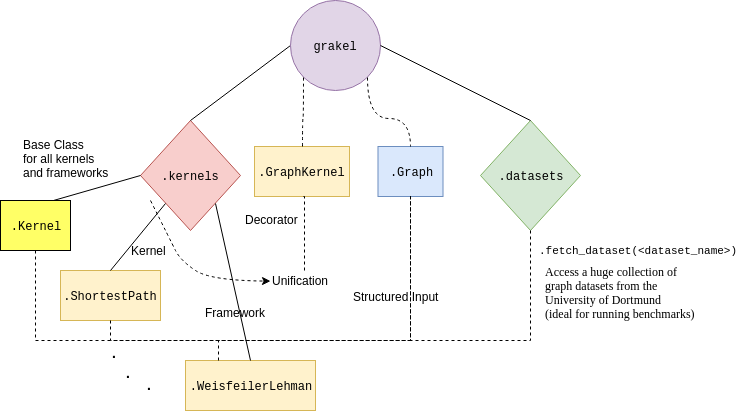
\includegraphics[width=\textwidth]{figures/grakel-schema}
    \caption[Σχηματική απεικόνιση της οργάνωσης του λογισμικού \en{grakel}]{Σχηματική απεικόνιση της οργάνωσης του λογισμικού \en{grakel}. Οι ρόμβοι αναπαριστούν υποπακέτα (\en{submodules}) ενώ τα παραλληλόγραμμα κλάσεις.}
    \label{fig:grakel}
\end{figure}
\section{Ανάπτυξη ενός Πυρήνα: Η κλάση \en{\texttt{Kernel}}}
Ας δούμε τώρα πιο αναλυτικά την σχεδίαση της κλάσης \en{\texttt{Kernel}} που αποτελεί την κύρια και σημαντικότερη οντότητα αυτής της βιβλιοθήκης (παράβαλε σχήμα \ref{fig:kernel_structure}).
Από την μελέτη της σχετικής βιβλιογραφίας ο υπολογισμός ενός γράφου πυρήνα μπόρεσε να αποδομηθεί στα εξής δύο αφηρημένα βήματα:  ($1$) ανάγνωση της εισόδου και εξαγωγή χαρακτηρηστικών και ($2$) υπολογισμός του πίνακα πυρήνα.
\subsection{Η Μέθοδος \texttt{\en{fit}}}
Κατά την κλήση της μεθόδου \texttt{\en{fit}} η βασική συνάρτηση η οποία καλείται είναι η \texttt{\en{parse\_input}} σχεδιασμένη για να φέρει εις πέρας το ($1$) και να αποθηκεύσει τα χαρακτηριστικά σε μία ιδιότητα της κλάσης.
Παράλληλα προκειμένου η κλάση \en{\texttt{Kernel}} να κληροομεί σωστά τον \en{\texttt{BaseEstimator}} ήταν αναγκαίο η μέθοδος \en{\texttt{set\_params}} να δουλεύει αποτελεσματικά, έπειτα από την αρχικοποίηση ενός αντικειμένου, ενώ ταυτόχρονα στην μέθοδο  \en{\texttt{\_\_init\_\_}} όλες οι παράμετροι εισόδου έπρεπε να αρχικοποιούν ιδιότητες με το ίδιο όνομα, για να δουλεύει η μέθοδος \en{\texttt{get\_params}}.
Ο έλεγχος μεταβλητών και η αρχικοποίηση δευτερευόντων χαρακτηριστικών ανατέθηκε στην συνάρτηση \texttt{\en{initialize\_}} η οποία καλείται στην πρώτη γραμμή της μεθόδου \texttt{\en{fit}}.

\subsection{Η Μέθοδος \texttt{\en{fit\_transform}}}
Για τον υπολογισμό της μήτρας πυρήνα είναι υπεύθυνες δύο μέθοδοι:\\ ($1$) η \texttt{\en{\_calculate\_kernel\_matrix}} και ($2$) η \texttt{\en{pairwise\_operation}}.
Στην περίπτωση του \texttt{\en{fit\_transform}} η πρώτη μέθοδος καλείται στο σύνολο των δεδομένων που έχουν αποθηκευθεί μετά την κλήση της μεθόδου \texttt{\en{parse\_input}} σε μία εσωτερική ιδιότητα της κλάσης \texttt{\en{self.X}}.
Τα δεδομένα αναμένεται να έχουν την μορφή ενός \texttt{\en{Iterable}}, το οποίο σε κάθε στοιχείο του περιέχει τα εξαχθέντα χαρακτηριστικά που αφορούν τον κάθε πυρήνα.
Χρησιμοποιώντας αυτά τα χαρακτηριστικά υπολογίζουμε την μήτρα πυρήνα, εφαρμόζοντας την μέθοδο \texttt{\en{pairwise\_operation}} μεταξύ κάθε ζευγαριού της άνω διαγωνίου (καθώς η μήτρα πυρήνα είναι πάντα συμμετρική).
Συνεπώς ο υπολογισμός της μήτρας πυρήνα κατανέμεται μεταξύ του υπολογισμού χαρακτηριστικών και της εφαρμογής μίας μετρικής μεταξύ τους.
Στις ακραίες περιπτώσεις (όπως συμβαίνει π.χ. με τα \en{\textit{R-frameworks}}) τα χαρακτηριστικά είναι τέτοια που ο υπολογισμός της μήτρας πυρήνα μπορεί να είναι ισοδύναμος με ένα γινόμενο πινάκων.
Όταν συμβαίνει κάτι τέτοιο, κατά την ανάπτυξη του πυρήνα είναι προτιμότερο να παραληφθεί η μέθοδος \texttt{\en{pairwise\_operation}} και να επανεγγραφεί η μέθοδος \texttt{\en{\_calculate\_kernel\_matrix}}.
Όσον αφορά την μέση περίπτωση που το υπολογιστικό κόστος κατανέμεται μεταξύ του συνήθως σειριακού \texttt{\en{parse\_input}} και του \texttt{\en{pairwise\_operation}} μία θεμελιώδης μέθοδος παραλληλοποίησης υλοποιήθηκε για τον υπολογισμό του πίνακα πυρήνα.
Συγκεκριμένα δεδομένου του πλήθους των στοιχείων της άνω διαγωνίου, ίσο με $\frac{N(N+1)}{2}$ και ενός πλήθους παράλληλων εργασιών \texttt{\en{n\_jobs}}, αν χωρίσουμε ομοιόμορφα τη λίστα δεικτών $K = [0, \dots, \frac{N(N+1)}{2}-1]$, μπορούμε έπειτα να πάρουμε τους δείκτες του ζητούμενου ζευγαριού γράφων $(i,j)$ που αντιστοιχούν σε ένα $k \in K$ ως:
\begin{align}
    i &= \left\lfloor N - 1 - \left\lfloor \frac{\sqrt{4N(N+1) - 8k - 7} - 1}{2}\right\rfloor \right\rfloor\\
    j &= \left\lfloor k + i - \left\lfloor \frac{N(N+1)}{2} \right\rfloor + \left\lfloor \frac{(N-i)(N-i+1)}{2} \right\rfloor \right\rfloor
\end{align}
Η υπολογιστική ωφελιμότητα της παραλληλοποίησης εξαρτάται από το υπολογιστικό κόστος της μεθόδου \texttt{\en{pairwise\_operation}} (σε σχέση με τις υπόλοιπες), πράγμα που μας απαγορεύει να την εγγυηθούμε στην γενική περίπτωση.

Στην περίπτωση που ο χρήστης επιθυμεί μία κανονικοποιημένη μήτρα πυρήνα η μέθοδος \texttt{\en{fit\_transform}} διαιρεί στοιχείο προς στοιχείο τις τιμές του πίνακα με την τετραγωνική ρίζα κάθε στοιχείου του εξωτερικού γινομένου της διαγωνίου με τον εαυτό της.
Η διαγώνιος του πίνακα πυρήνα αποθηκεύεται σε κάθε περίπτωση σε μία εσωτερική μεταβλητή προκειμένου να μπορεί να χρησιμοποιηθεί χωρίς να επανυπολογιστεί κατά την κλήση της μεθόδου \texttt{\en{diagonal}}.
\subsection{Η Μέθοδος \texttt{\en{transform}}}
Όσον αφορά τώρα την περίπτωση του \texttt{\en{transform}} όλες οι μέθοδοι που αναφέρθηκαν παραπάνω θα πρέπει να προσαρμοστούν.
\begin{figure}[]
    \centering
    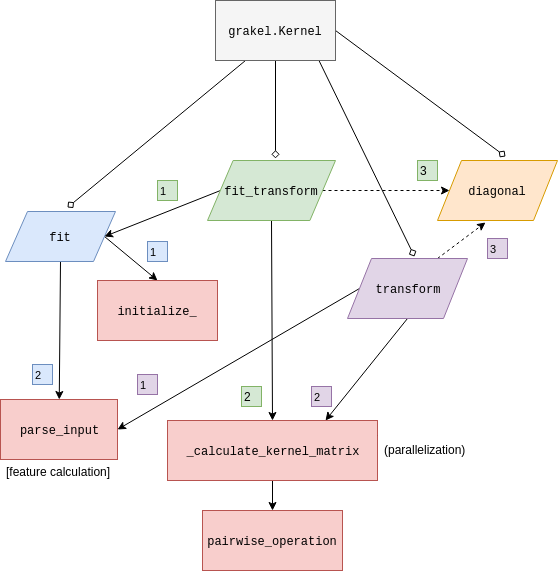
\includegraphics[width=0.6\textwidth]{figures/KernelStructure.png}
    \caption[Σχηματική απεικόνιση του τρόπου οργάνωσης των μεθόδων της κλάσης \en{\texttt{Kernel}}.]{Σχηματική απεικόνιση του τρόπου οργάνωσης των μεθόδων της κλάσης \en{\texttt{Kernel}}. Τα νούμερα συμβολίζουν την σειρά κλήσης άλλων μεθόδων από την εκάστοτε μέθοδο. Η διακοπτόμενη κλήση αφορά την περίπτωση που κατά την αρχικοποίηση η παράμετρος \en{normalization} είναι \en{\texttt{True}}.}
    \label{fig:kernel_structure}
\end{figure}
Συγκεκριμένα σε πρώτη φάση, το \texttt{\en{parse\_input}} καλείται να σχηματίσει χαρακτηριστικά συγκρίσιμα με τα δεδομένα του \texttt{\en{fit}}.
Σε πολλές περιπτώσεις κάτι τέτοιο απαιτεί την αποθήκευση μετα-πληροφορίας κατά το \texttt{\en{fit}} (π.χ. ενός λεξικού που λειτουργεί ως αρίθμηση των επισημειώσεων) αλλά και της δυνατότητας του \texttt{\en{parse\_input}} να γνωρίζει αν καλείται από το \texttt{\en{transform}}, το \texttt{\en{fit}} ή και σε κάποιες περιπτώσεις από το \texttt{\en{fit\_transform}}.
Κάτι τέτοιο επιλύεται φυσικά με την χρήση μία ιδιωτικής ιδιότητας \texttt{\en{self.\_method\_calling}} της κλάσης, που λαμβάνει τιμές $1, 2, 3$ κατά τα \texttt{\en{fit}}, \texttt{\en{fit\_transform}} και \texttt{\en{transform}} αντίστοιχα.
Εν συνεχεία κατά την κλήση της συνάρτησης \texttt{\en{\_calculate\_kernel\_matrix}} μεταξύ όλων των ζευγαριών των δεδομένων του \texttt{\en{transform}} και του \texttt{\en{fit}}, τρέχουμε την μέθοδο \texttt{\en{pairwise\_operation}}.
Σε αυτήν την περίπτωση, δεδομένου ενός πλήθους παράλληλων εργασιών \texttt{\en{n\_jobs}} η παραλληλοποίηση επιτυγχάνεται αν χωρίσουμε ομοιόμορφα την λίστα δεικτών $K = [0, \dots, Ν Μ - 1]$ (όπου $Μ$ το πλήθος των δεδομένων κατά το \texttt{\en{transform}}), και έπειτα για κάθε $k \in K$ εξάγουμε για κάθε επεξεργαστή τα ζευγάρια δεικτών $(i,j)$ ως $(k\mod N, \lfloor \frac{k}{N} \rfloor)$.\par
Στην περίπτωση που ο χρήστης επιθυμεί μία κανονικοποιημένη μήτρα πυρήνα η μέθοδος \texttt{\en{transform}} καλεί την μέθοδο \texttt{\en{diagonal}} η οποία επιστρέφει το διάνυσμα της τιμής πυρήνα όλων των στοιχείων του \texttt{\en{fit}} με τον εαυτό τους $d_{x}$, καθώς και το διάνυσμα της τιμής πυρήνα όλων των στοιχείων του \texttt{\en{transform}} με τον εαυτό τους $d_{y}$.
Προκειμένου να προκύψει ο κανονικοποιημένος πίνακας, διαιρεί στοιχείο προς στοιχείο της $Μ \times N$ μήτρας πυρήνα με την τετραγωνική ρίζα κάθε στοιχείου του εσωτερικού γινομένου $d_{y} \times d_{x}$.


\section{\en{Packaging}}
Έκτος από την ίδια την σχεδίαση (\en{design}) και την ανάπτυξη (\en{development}) της, η ολοκλήρωση μίας σύγχρονης βιβλιοθήκης προγραμματισμού απαιτεί την \textit{συσκευασία} της (\en{packaging}).
Αν μία βιβλιοθήκη μπορεί να παρομοιαστεί με ένα μηχανισμό, σε επίπεδο ανάπτυξης ένας προγραμματιστής πρέπει να μπορεί να αναγνωρίσει τα δομικά της μέρη, να μπορεί να καταλάβει από τι αποτελούνται, πως κατασκευάζονται και τον τρόπο με τον οποίο συναρμολογούνται, καθώς και να μπορεί να ανιχνεύσει τις αλλαγές της από το παρελθόν, ενώ δύναται γνωρίζοντας λεπτομερώς μέρη από την παρούσα μορφή της να την διορθώσει ή να την επεκτείνει.
Σε επίπεδο χρήσης, η γνώση της έκδοσης της και η γενική \textit{επαλήθευση λειτουργίας} της, η ευκολία εγκατάστασης της, η δυνατότητα ελέγχου λειτουργίας χωρίς την γνώση χρήσης της, καθώς και η διάθεση ενός εγχειριδίου που περιέχει πληροφορίες σχετικές με την εγκατάσταση, την χρήση και την κατασκευή της είναι εξίσου απαραίτητα.
Παρόλο που συχνά στο εύρος των ατόμων που απευθύνονται τέτοιες βιβλιοθήκες οι δύο αυτοί ρόλοι, \textit{προγραμματιστή} και \textit{χρήστη} είναι ζήτημα "εστίασης της προσοχής", είναι χρήσιμο να συντηρούνται ως πόλοι ανάπτυξης του λογισμικού.
\subsection{Ανάπτυξη Κώδικα}
Ξεκινώντας από την ανάπτυξη κώδικα σημαντικό είναι να ξεκινήσουμε με τους βασικούς κανόνες συγγραφής του.
\subsubsection{Το Πρότυπο \en{PEP-8}}
Προκειμένου ο κώδικας να είναι ευανάγνωστος, η ανάπτυξη κάθε πακέτου προγραμματισμού \en{python} καλείται να ακολουθεί συγκεκριμένους ``αισθητικούς'' κανόνες τόσο στο επίπεδο της σύνταξης όσο και της σημασιολογίας.
Το πρότυπο \en{PEP-8} είναι το παρόν πρότυπο σύνταξης για την γλώσσα προγραμματισμού \en{Python}.
Περιέχει κανόνες που αφορούν το μέγιστο δυνατό μήκος μίας γραμμής κώδικα και την στοίχιση των ορισμάτων κατά την κλήση ή τον ορισμό μίας συνάρτησης, που επεκτείνονται πέραν της μίας γραμμής, μέχρι κανόνες για τον τρόπο ελέγχου ενός τύπου, τον τρόπο χειρισμού εξαιρέσεων (\en{exception handling}) και την χρήση συναρτήσεων αντί για συναρτησιακών (\en{lamda's}) \cite{PEP8}.
Το πρότυπο αυτό μπορεί να παραμετροποιείται από τον εκάστοτε προγραμματιστή, αλλά εξασφαλίζει μία συνοχή στον τρόπο με τον οποίο τελικά συντάσσει κώδικα.
Για τον αυτόματο έλεγχο του παραπάνω, έχει αναπτυχθεί ένα αντίστοιχο πακέτο γνωστό ως \href{https://pypi.org/project/flake8/}{\en{flake8}}.
\subsubsection{\en{PyPI}}
Κάθε πακέτο \en{python} απαιτεί να μπορεί να εγκατασταθεί οικουμενικά σε όλο το σύνολο των μηχανημάτων για τα οποία προορίζεται.
Κάτι τέτοιο επιλύεται μέσω της ίδιας της \en{python} (βλ. βιβλιοθήκη \href{https://pypi.org/project/setuptools/}{\en{setuptools}}) και απαιτεί από τον προγραμματιστή μονάχα ένα στοιχειώδη τρόπο οργάνωσης της βιβλιοθήκης, καθώς και την συγγραφή ενός αρχείου εγκατάστασης \en{setup.py}.
Διαθέτοντας κάτι τέτοιο η βιβλιοθήκη μπορεί να τοποθετηθεί στο ηλεκτρονικό αποθετήριο βιβλιοθηκών της \en{Python}, γνωστό ως \en{PyPI: \textbf{Py}thon \textbf{P}ackage \textbf{I}ndex}, μέσω του οποίου μπορεί να εγκατασταθεί από το κύριο εργαλείο εγκατάστασης βιβλιοθηκών, γνωστό ως \href{https://pypi.org/project/pip/}{\en{pip}}.
Η \en{python} ως γλώσσα με διερμηνέα δεν διαθέτει την έννοια των εκτελεσίμων όπως αυτή υπάρχει από την \en{C} (\en{binaries}) ή την \en{Java} (\en{bytecode}), ταυτίζοντας το πακέτο εκτέλεσης με τον ίδιο τον κώδικα, μέσω των λεγόμενων \en{\textit{eggs}}.
Για να καλυφθεί αυτή και άλλες ανάγκες, τα λεγόμενα \href{https://pythonwheels.com/}{\en{wheels}} εισήχθησαν από την κοινότητα που αναπτύσσει την γλώσσα \en{python}.\par
Περαιτέρω, κάθε σύγχρονη βιβλιοθήκη επιστημονικού υπολογισμού (\en{scientific-computing}) καλείται να μπορεί συνταιριάξει, το ευχάριστο και μή-περιοριστικό προγραμματιστικό της περιβάλλον, με τα άγρια και άκομψα πλάσματα των γλωσσών \en{C, C++, Fortran} λόγω της αμεσότητας και της αποδοτικότητάς τους.
Τόσο στο επίπεδο του \en{setup.py} όσο και στο επίπεδο των \en{wheels} κάτι τέτοιο δεν αποτελεί μία δυσπρόσιτη πρακτική, ειδικά με την χρήση πακέτων όπως το \href{https://pypi.org/project/Cython/}{\en{Cython}}.
Τέλος σημαντικό για τον έλεγχο κάθε πακέτου είναι η ύπαρξη ενός συνόλου από στοιχειώδη δοκιμαστικά προγράμματα (\en{unit-tests}) προκειμένου πριν την δημοσίευση του κώδικα, αλλά και κατά την συντήρηση και επέκταση του να επαληθεύεται η σωστή λειτουργία του.
Πακέτα όπως το \href{https://pypi.org/project/nose/}{\en{nose}} έχουν αναπτυχθεί, προκειμένου η εκτέλεση και η καταγραφή των προβλημάτων που προκύπτουν από την εκτέλεση τους να παρουσιάζεται συνοπτικά, ενώ ενσωματώνουν άλλα όπως το \href{https://pypi.org/project/coverage/}{\en{coverage}} που είναι υπεύθυνο να παρουσιάζει στατιστικά στοιχεία, σχετικά με τον βαθμό στον οποίο τα δοκιμαστικά προγράμματα δοκιμάζουν τον πλήρη κώδικα της βιβλιοθήκης.

\subsection{Δημοσίευση Κώδικα}
Όπως προαναφέρθηκε για την δημοσίευση του κώδικα της παρούσας βιβλιοθήκης χρησιμοποιήθηκε το ηλεκτρονικό αποθετήριο \href{https://github.com/}{\en{GitHub}}, παράλληλα με το γεγονός ότι οι εκδόσεις του καταγράφονται μέσω του συστήματος \en{git}.
Απαραίτητα όμως για την δημοσίευση του παρόντος λογισμικού επιστημονικού υπολογισμού \en{python} είναι η ύπαρξη \en{Documentation}, η συνεχή του ενσωμάτωση (\en{Continuous Integration}) καθώς και η άδεια του.
\subsubsection{\en{Documentation}}
Ίσως το πιο σημαντικό βήμα τόσο όσον αφορά τον χρήστη, αλλά και τόσο όσον αφορά τον προγραμματιστή που αναπτύσσει την βιβλιοθήκη, είναι η συγγραφή ενός εγχειριδίου γνωστό με τον όρο \textit{\en{documentation}}.
Από την ίδια την αναλυτική καταγραφή των κλάσεων, την όμορφη παρουσίαση του κώδικα και τις οδηγίες εγκατάστασης, ένα εγχειρίδιο μπορεί να αποτελείται από πολλά περισσότερα μέρη όπως εισαγωγικό κείμενο για την χρήση της βιβλιοθήκης, θεωρητική ανάλυση των απαραίτητων μεθόδων της, πληροφορίες σχετικά με την επέκταση της, και πιο ενδιαφέροντα παραδείγματα χρήσης της.
Η πραγμάτωση όλων των παραπάνω αυτοματοποιείται όσον αφορά την παρουσίαση των κλάσεων και του κώδικα (μέσω κατάλληλης σύνταξης στο επίπεδο των σχολίων) και διευκολύνεται όσον αφορά τα υπόλοιπα, παράγοντας ένα ευχάριστο αισθητικό αποτέλεσμα μέσω του πακέτου \href{https://pypi.org/project/Sphinx/}{\en{Sphinx}}.
\subsubsection{Συνεχής Ενσωμάτωση}
Κάθε νέα έκδοση ενός λογισμικού η οποία προστίθεται στο ηλεκτρονικό αποθετήριο \texttt{\en{GitHub}} πρέπει να συνδέεται με μία εγγύηση ότι αυτή η έκδοση είναι λειτουργική.
Κάτι τέτοιο αποτελεί μία καθιερωμένη πρακτική τα τελευταία χρόνια, μέσω των πλατφορμών συνεχούς ενσωμάτωσης (\en{continuous integration}) οι οποίες επιτρέπουν την ολιγόχρονη αρχικοποίηση ενός λειτουργικού συστήματος και τον προγραμματισμό μία σειράς βημάτων, μέσω της οποίας μπορούν να ελέγχονται αυτόματα αν έρχονται εις πέρας, η κατάλληλη παραμετροποίηση του συστήματος, η εγκατάσταση και η δοκιμή της βιβλιοθήκης, κάθε φορά που μία νέα έκδοση προστίθεται στο ηλεκτρονικό αποθετήριο.
Συγκεκριμένα ο έλεγχος της βιβλιοθήκης \en{GraKeL} γίνεται σε λειτουργικό σύστημα \en{Linux} και \en{OSX} μέσω της πλατφόρμας συνεχούς ενσωμάτωσης \href{https://travis-ci.org/ysig/GraKeL}{\en{Travis}} και σε λειτουργικό σύστημα \en{Windows} μέσω της πλατφόρμας \href{https://ci.appveyor.com/project/ysig/grakel}{\en{Appveyor}}.
Μιας και αυτά τα περιβάλλοντα είναι στοιχειώδη (\en{minimal}) και η βιβλιοθήκη κάτι αφηρημένο σε σχέση με το ίδιο το λειτουργικό σύστημα η εγγύηση λειτουργίας τους σε όλες τις υποστηριζόμενες εκδόσεις \en{Python} είναι συνήθως ανεξάρτητη από την έκδοση του λογισμικού (παρόλο που δίνεται η δυνατότητα ορισμού του).
Επιπλέον οι πλατφόρμες αυτές χρησιμοποιήθηκαν για την ανάπτυξη και απόθεση (\en{build and deploy}) \en{wheels} για ένα εύρος συστημάτων και όλες τις υποστηριζόμενες εκδόσεις \en{python} στο \en{PyPi}, μέσω της βιβλιοθήκης \href{https://github.com/joerick/cibuildwheel}{\en{cibuildwheel}}.
Τέλος, μία τρίτη πλατφόρμα χρησιμοποιήθηκε για την ανάπτυξη και απόθεση του \en{documenation}, συγκεκριμένα η \href{https://circleci.com/gh/ysig/GraKeL/tree/develop}{\en{Circle-CI}}.
Η λειτουργικότητα τις βιβλιοθήκης όπως επισημαίνεται από τα παραπάνω καθώς και το ποσοστό του \en{coverage} όπως αυτό αποτίθεται στην πλατφόρμα \href{https://codecov.io/gh/ysig/GraKeL}{\en{codecov}} μέσω του \en{travis}, φαίνονται με την μορφή \en{badges} στην κύρια σελίδα στο αποθετήριο του \href{https://github.com/ysig/GraKeL}{\en{GraKeL}}.

\subsubsection{Άδεια}
Είναι καθιερωμένο για κάθε επίσημα δημοσιοποιημένο λογισμικό να κατέχει μία άδεια χρήσης.
Για την δημοσίευση του \en{GraKeL} επιλέχθηκε η ίδια άδεια χρήσης με αυτή του \href{https://en.wikipedia.org/wiki/Scikit-learn}{\en{scikit-learn}}, συγκεκριμένα η \href{https://en.wikipedia.org/wiki/BSD_licenses#3-clause_license_(%22BSD_License_2.0%22,_%22Revised_BSD_License%22,_%22New_BSD_License%22,_or_%22Modified_BSD_License%22)}{άδεια \en{BSD} 3 ρητρών}.
Η άδεια αυτή είναι μία άδεια αποδεκτή από την κοινότητα ελευθέρου λογισμικού (\en{FSF-approved}), με τρία στοιχειώδη απαιτούμενα.
Συγκεκριμένα, την επανατοποθέτηση αυτής της άδειας σε αναδιανομές του λογισμικού τόσο αν αυτές είναι σε μορφή κώδικα ή εκτελέσιμου, καθώς και την διαφύλαξη των μελών του προσώπου δικαίου που φέρει τα πνευματικά δικαιώματα, από την χρήση των ονομάτων τους για την πρόκριση ή την προώθηση παραγώγων αυτού του λογισμικού, χωρίς να έχει προηγηθεί η γραπτή τους άδεια.
